% Chapter Template

\chapter{Implementation} % Main chapter title

\label{Chapter5} % Change X to a consecutive number; for referencing this chapter elsewhere, use \ref{ChapterX}

%----------------------------------------------------------------------------------------
%	SECTION 1
%----------------------------------------------------------------------------------------

\section{Data collection and cleaning}

The key foundation of the project was being able to collect the data that would allow the creation of the well-being domain scores. Collecting the required data and shaping it into the formats that were needed was, in places, one of the most challenging aspects of the project and the one that required the largest proportion of time. This part of the project presented several challenges that needed to be overcome.

%-----------------------------------
%	SUBSECTION 1
%-----------------------------------
\subsection{Collection of data files}

For ward level data, the Greater London Authority's datastore is a primary data source. A significant proportion of the data for the creating of the well-being indicators could be accessed via this source. 

%-----------------------------------
%	SUBSECTION 2
%-----------------------------------

\subsection{Collection from APIs}

The API that was key to the success of the project was that of social media platform Foursquare. To represent community vitality, the aim was to create a measure for the restaurants and bars in each ward. Foursquare is a platform based around venue information so holds the information required for this measure. Foursquare also holds information on cultural venues. Therefore the measure of 'Access to Cultural Space' could also be obtained from this platform.
To use the API to obtain venue information you are required to search for venues within a specified radius of a certain point, given in latitude and longditude. The challenge with Foursquare was the the API rate limits which limits each search to a maximum of 49 searches. There are also daily and monthly rate limits to stay within.
To obtain results of all bars, restaurants and cultural venues accross Greater London with these limits an iterative algorithm had to be created which could travel accross London by latitude and longditude, taking in small enough areas so as to not exceed 49 results a time. This function can be seen in figure ~\ref{fig:pyimpfsq}. To achieve this, a latitude and longditude bounding box was created around London and a nested loop iteration of 50 points of latitude and 50 points of longditude was undertaken. The areas created by this had some overlap so as not to have missing areas of the capital. With a counter to check if the search limit of 49 venues was exceeded, this search algorithm put the list of venues into a pandas dataframe and de-duplicated for where areas had ovelapped.


\begin{figure}
\centering
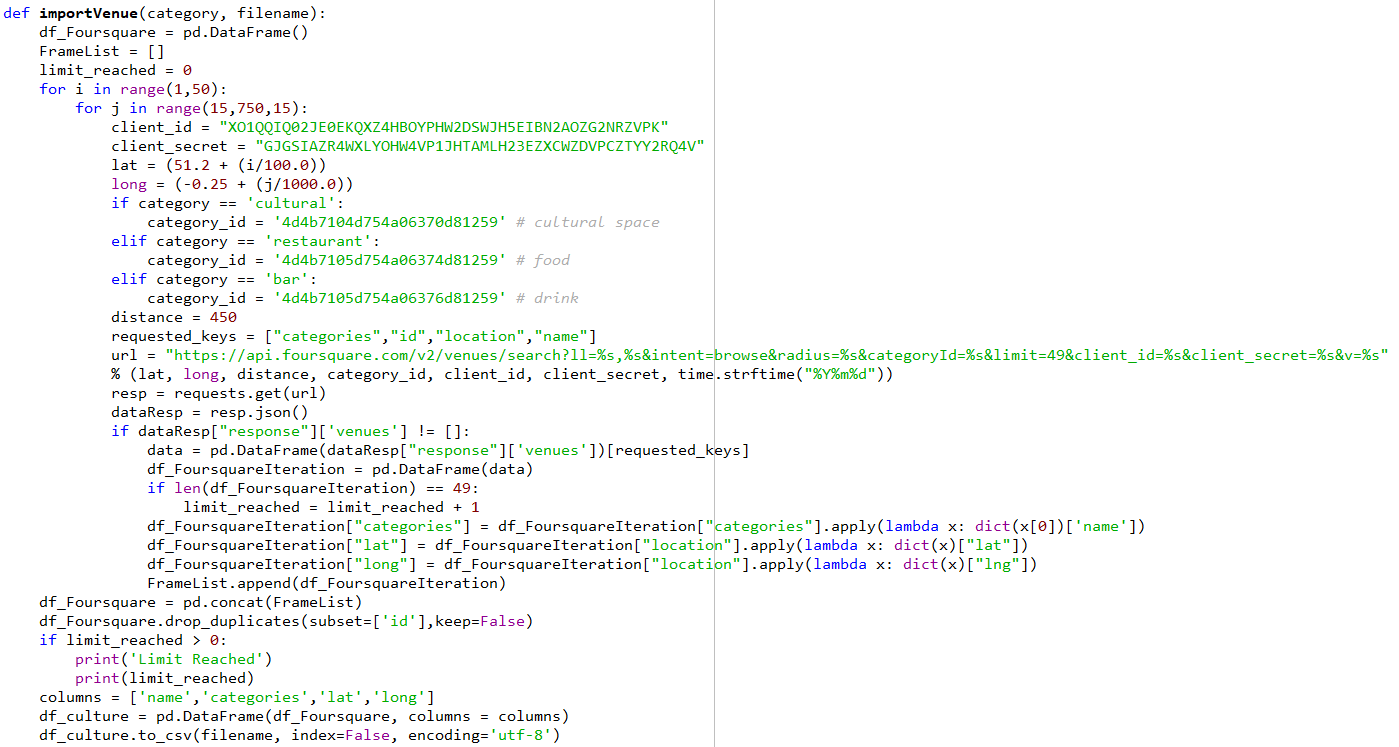
\includegraphics[scale=0.6]{figures/API_import}
\decoRule
\caption{Python function written to import data from Foursquare. This function iterates for latitude and longitude to traverse London and return venue information for one of three categories ("cultural", "food" or "nightlife) without exceeding daily API limits.}
\label {fig:pyimpfsq}
\end{figure}

Because of the rate limits, running the algorithm for such a large area could only be done on a daily basis.

%----------------------------------------------------------------------------------------
%	SECTION 2
%----------------------------------------------------------------------------------------

\section{Well-being domain scores}

The motivation for creating composite domain scores 6 different measures of well-being was two-fold. Firstly creating a score for each domain over a pre-defined scale would allow users of the front-end interactive map compare scores accross wards and give those scores some contextual meaning and significance. With 6 domains rather than the original 18 datasets, the amount of information presented to the user would not be too large to prevent a non-technical audience from interpreting the information on the map. The second reason for creating the domain indicators was to help to try and create an interpretable model rather than one requiring significant dimension reduction. Whilst some less interpretable models will be tested to validate the quality of the quintile classification model, ideally the project and the user front end should allow us to draw some conclusions about any link between well-being and median house prices in London.

For each domain three appropriate datasets were chosen and then reduced to give a single score for each ward. The 3 datasets for each domain were standardised using a function in Python and those which related to a negative indicator such as emissions or crime were mutliplied by a value of -1. Using this technique of standardisation gave equal weighting to each of the three indicators. Because of the equal weighting given to each indicator, these can be seen as substitutable within the context of the domain which is a important factor in the choice of technique used to reduce the indicators to a score. With indicators that can be assumed to be substitutable suitable techniques would include Principal Component Analysis (PCA) and an arithmetic mean
?INSERT REFERENCE TO PAPER BY ITALIAN ACADEMICS?
For the 6 domains, a mixture of the two techniques have been used. For those domains where the 3 indicators have a relatively high correlation ?ABOVE WHAT? the first Principal Component has been used to try and extract the largest amount of variance within the three indicators. Where the indicators for a domain have low levels of correlation for at least one of the three datasets, the arithmetic mean has been used. This approach gives us three domains which use PCA and three which use the mean.
?INSERT COV MATRICES AND TECHNIQUES FOR EACH DOMAIN?
This approach tries to maximise the information contained in all of the datasets.
To create an interpretable and comparable score for each domain the resulting single scores have been normalised and then rescaled to be between 0 and 100, this is the score that is presented in the user front end.


%----------------------------------------------------------------------------------------
%	SECTION 3
%----------------------------------------------------------------------------------------

\section{Building a regression model}

To begin the task of trying to model the median house prices from the well-being indicces, a simple multiple linear regression model was used with all six indices as predictors. The results show that this model explains less than half the variance with an R squared value of 0.39. There is enough to suggest that some form of linear model may provide a reasonable model of this problem.
To validate the model K-fold cross validation was used with k=7 with accuracy scores and mean squared errors average accross the seven iterations.

The summary statistics for a simple linear model would suggest some level of statistical significance for all of the indices with Community Vitality and Participation and Education and Employment less significant than the others. Infrastructure and Health are the most significant indices here and they are also the most influential on the model. Safety and Security is the only index where there is a negative impact on house prices in the model. 

\begin{table}[H]
\caption{Results for regression models on London median house prices}
\centering
\begin{tabular}{lllll}
\toprule
Predictor               & coef    & std err & t      & p     \\
\midrule
const                   & 46.9752 & 135.66  & 0.346  & 0.729 \\
Education\_Employment   & 1.4541  & 0.759   & 1.915  & 0.056 \\
Safety\_Security        & -4.5924 & 1.391   & -3.301 & 0.001 \\
Environment             & 2.0667  & 0.712   & 2.902  & 0.004 \\
Vitality\_Participation & 2.2165  & 1.227   & 1.807  & 0.071 \\
Infrastructure          & 9.2899  & 0.769   & 12.075 & 0     \\
Health                  & 6.2779  & 0.624   & 10.064 & 0  \\
\bottomrule\\  
\end{tabular}
\end{table}

Next a polynomial model was tried with degree two. This model explained almost none of the variance with an R sq value of very close to 0. The mean squared error also increased dramatically. The polynomial model does not seem to be a strong candidate for solving the problem.

The next models involved some feature reduction based on the p values of the indices in the original linear model. This meant that first Education and Employment were removed and then Community Vitality and Participation. This resulted in a small improvement in the model fit but little improvement in the MSE. 

With the median house price distribution suggesting a power law, a log transformation was performed on the data to try and linearise it with the linear regression model then re-run. This transformation dramatically increased the R sq value of the model, to 0.64, an increase of 0.25 from the equivalent model without the transformation. The model run on the log transformed data explains an additional 25 percent of the variance within the model. The exponent of the MSE is also a substantial reduction. This returned the following model:

\begin{equation}
\resizebox{.8\hsize}{!}{$log(Median_Price) = 0.00300393*I1 + 0.00201057*I2 + 0.00191012*I3 +0.0081844*I4 + 0.01301158*I5 + 0.00742296*I6$}
\end{equation}

where I1 = Education and Employment, I2 = Safety and Security, I3 = Environment, I4 = Community Vitality and Participation, I5 = Infrastructure and I6 = Health

The equation shows that Infrastructure has the largest impact on the median house prices in the model followed by Community Vitality and Participation and then Health. All indices have a positive impact on median house prices in the model, Environment is the least influential index

As the best performing regression model this will be used for prediction in the final visulisation.

When the predictions were given the inverse transformation and validated against the actual values, the majority of wards showed that this model had good predictive capability although there were a handful of wards where the prediction had a signifcant error margin. The wards with significant errors tended to be those which had a much higher or lower score in a particular domain as compared to the neighbouring areas.

\begin{table}
\caption{Results for regression models on London median house prices}
\centering
\begin{tabular}{l l l}
\toprule
Model & R squared & Average MSE \\
\midrule
Linear regression & 0.396 & 35326.75\\
Linear regression with  polynomial degree 2 & 0.007 & 59013.81\\
Linear regression with 5 dimensions & 0.473 & 33907.16\\
Linear regression with 4 dimensions & 0.443 & 34608.08\\
Linear regression on log-transformed data & 0.641 & 4944.06\\
\bottomrule\\
\end{tabular}
\end{table}


%----------------------------------------------------------------------------------------
%	SECTION 4
%----------------------------------------------------------------------------------------

\section{Building the best classifier}

The first model investigated was a logistic regression model. With strong interpretability well-performing logistic regression model would provide a good solution to the problem.
The model had a classification success rate of 44 percent, showing a reasonable level of predictive capability across a five value classification problem. The confusiion matrices provided by the seven cross-validation iterations show that model performs strongly in the first and fifth quintiles but finds it much more difficult to classify points in the second, third and fourth quintiles.
From the pair-wise plots ? OR USE BOXPLOT? this is unsurprising as the range of median house prices is much smaller for the middle three quintiles and many of the well-being indicators are of similar magnitude.

For the second model a k-nearest neighbours classifier was used, this achieved a 40 percent classification success rate and was outperformed by the logistic regression model.

A model using a Gaussian Naive Bayes algorithm performed very slightly above the logistic regression, however, given the better interpretability of the logistic regression model, the 0.2 percent gain would not be enough to justify using this model for the solution.

The next model investigated was a decision tree, with an average classification percentage of 38, this performed significantly below the rate of the logistic regression model.

Although a single decision tree was the worst of the classifiers used so far, the next models investigated were ensemble models. A random forest was tried on the data. With 10 trees this performed below the level of the logistic regression model, but when tuned to use 100 trees, this produced the best classification score so far at just under 46 percent. The random forest was therefore a candidate to use as the classification model.
Another ensemble method, gradient boosting, also performed better than the logistic regression model but was not able to match the random forest's correct classification rate.

The final model used was a Neural Network using a single hidden layer. A process of tuning this model involved trying four activation functions, of which the logistic function performed best. Different values were used for the number of nodes in the hidden layer with 45 giving the highest classification rate.
By using a tuned Neural Network, a 50 percent classification rate was achieved. This was a significant improvement on the other models used.

\begin{table}[]
\caption{Results for Neural Network classifier with Logistic activation function and different numbers of nodes in the hidden layer. Based on average scores using k-fold cross validation with k=7.}
\centering
\begin{tabular}{ll}
\toprule
Number of nodes in hidden layer & Test Score \\
\midrule
5                               & 0.469      \\
10                              & 0.477      \\
15                              & 0.474      \\
20                              & 0.490      \\
25                              & 0.458      \\
30                              & 0.471      \\
35                              & 0.482      \\
40                              & 0.451      \\
45                              & 0.502      \\
50                              & 0.488      \\
55                              & 0.498      \\
60                              & 0.496      \\
65                              & 0.483      \\
70                              & 0.501      \\
75                              & 0.482      \\
80                              & 0.480      \\
85                              & 0.456      \\
90                              & 0.490      \\
95                              & 0.471      \\
100                             & 0.490     \\
\bottomrule\\
\end{tabular}
\end{table}

\begin{table}[]
\caption{Results for Neural Network classifier with 45 nodes in the hidden layer and different activation functions. Based on average scores using k-fold cross validation with k=7.}
\centering
\begin{tabular}{ll}
\toprule
Activation Function & Test Score \\
\midrule
identity            & 0.380 \\
logistic            & 0.485 \\
tanh                & 0.445 \\
relu                & 0.446    \\
\bottomrule\\
\end{tabular}
\end{table}


To take advantage of both interpretability and classification success rates, it was decided to display the predicted quintile values for both the Logistic Regression model and the Neural Network in the final map visualisation. 
The results of testing each of the different models using k-fold cross validation with k=7 were:

\begin{table}
\caption{Results for classification models on the quintiles of London median house prices}
\centering
\begin{tabular}{lll}
\toprule
Model Type           & Training Score & Test Score \\
\midrule
Logistic Regression  & 0.470          & 0.440      \\
Decision Tree        & 1.000          & 0.388      \\
K-Nearest Neighbours & 0.614          & 0.407      \\
Random Forest        & 1.000          & 0.459      \\
Gradient Boosting    & 0.987          & 0.448      \\
Naive Bayes          & 0.465          & 0.442   \\  
\bottomrule\\
\end{tabular}
\end{table}

%----------------------------------------------------------------------------------------
%	SECTION 5
%----------------------------------------------------------------------------------------

\section{Encoding as geoJSON}

To use the information from the creation of the well-being domains and the predictions obtained from the models in a javascript based visualisation, the information needed to be converted from a pandas dataframe in Python to a geoJSON file in javascript. A geoJSON file is a variation on the JSON format as defined below:

\begin{figure}
\centering
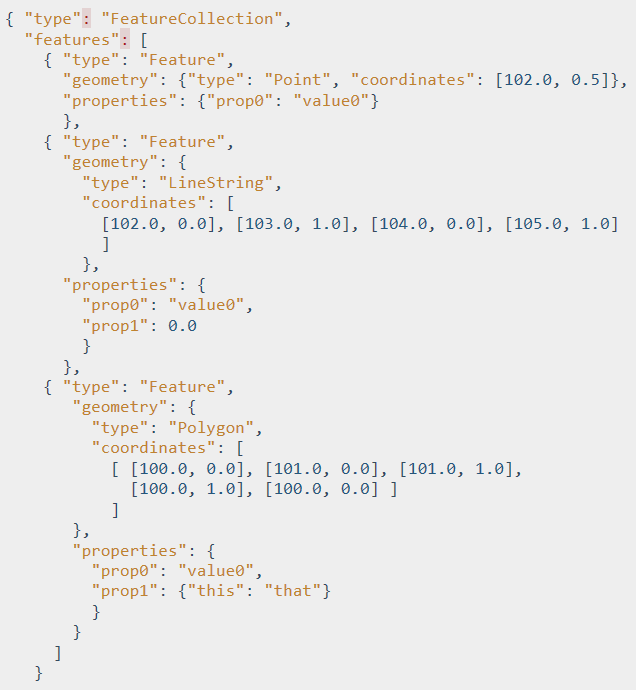
\includegraphics[scale=0.7]{figures/geoJSON}
\decoRule
\caption{geoJSON specification showing Point, LineString and Polygon geometry objects.}
\end{figure}

Whilst a relatively straightforward task within the geopandas module in Python, geoJSON accepts coordinates in latitude and longditude and the shapefile being used has the coordinates defining the ward polygons in Ordnance Survey grid references. To change this to latitude and longditude required the creation of a function that would take each polygon in the ward geometry in the geo data frame and break this down into the individual points which define the polygon. Once separated into coordinate pairs, these pairs could be reprojected to be latitude and longditude. The function was then required to recombine all of the coordinate pairs into the correct polygon geometries.

? CODE SNIPPET?

The information was then in the required format to be exported to a geoJSON file.

%----------------------------------------------------------------------------------------
%	SECTION 6
%----------------------------------------------------------------------------------------

\section{Interactive maps}

For the production of the interactive map which serves as the user front end for this project, the information was moved from the Python environment via geoJSON and into javascript functions embedded into html. This decision was made on the basis of the additional functionality and interactivity that could be smoothly added to the map in javascript. With less experience of javascript as a programming language, the leaflet.js tutorial (\cite{leaflet}) was an excellent starting point.

The map has key functionality added. This includes a zoom facility and hovering over any of the 625 wards will display the median house price value and quintile, the scores for each of the six well-being domains and the predictions from both the regression and classification models.







